Il seguente listato genera due grafici per le funzioni date:
\lstinputlisting[language=Matlab]{cap_4/es2/es2.m}
\lstinputlisting[language=Matlab]{cap_4/es2/evaluate_poli.m}
\global\csname @topnum\endcsname 0
\begin{figure}
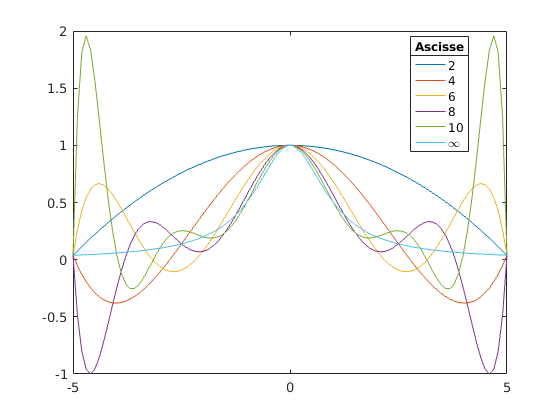
\includegraphics[scale=0.7]{cap_4/es2/Runge_equi.png}
\caption{Ascisse Equidistanti per $f(x) = \frac{1}{1+x^2}$}
\label{RungeEq}
\end{figure}
\begin{figure}
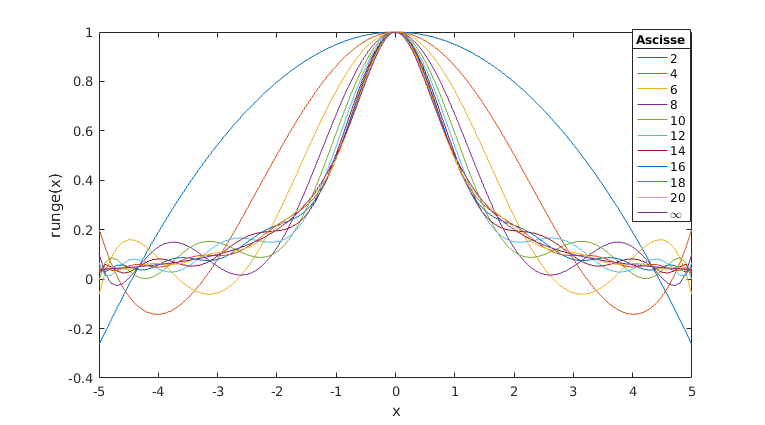
\includegraphics[scale=0.7]{cap_4/es2/Runge_cheb.png}
\caption{Ascisse di Chebyshev per $f(x) = \frac{1}{1+x^2}$}
\label{RungeChe}
\end{figure}
\begin{figure}
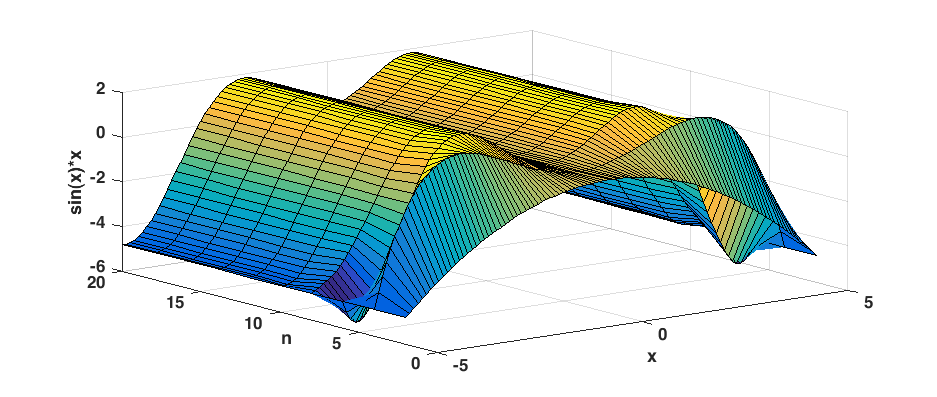
\includegraphics[scale=0.7]{cap_4/es2/Sin_equi.png}
\caption{Ascisse Equidistanti per $g(x) = sin(x)*x$}
\label{SinEq}
\end{figure}
\begin{figure}
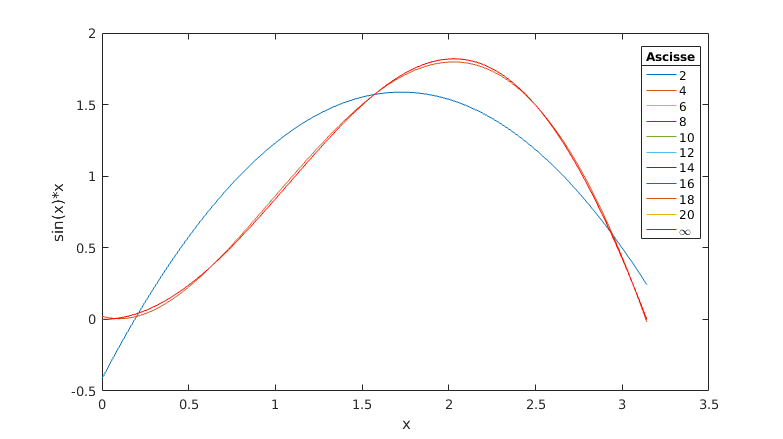
\includegraphics[scale=0.7]{cap_4/es2/Sin_cheb.png}
\caption{Ascisse di Chebyshev per $g(x) = sin(x)*x$}
\label{SinChe}
\end{figure}
\begin{figure}
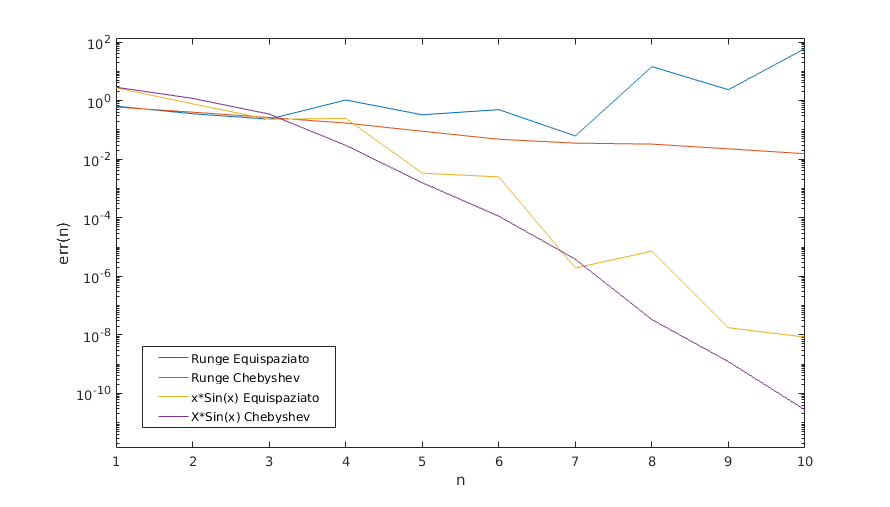
\includegraphics[scale=0.7]{cap_4/es2/error.png}
\caption{Confronto degli errori per le due funzioni}
\label{error}
\end{figure}
Possiamo vedere la differenza tra \ref{RungeEq} e \ref{RungeChe}, nella prima all'aumentare delle ascisse la funzione interpolata degenera, mentre nella seconda già con n=5 abbiamo una buona interpolazione.
Nel caso della seconda funzione possiamo vedere che la differenza tra \ref{SinEq} e \ref{SinChe} non è molto rilevante.
L'ultima figura \ref{error} è un confrontro tra gli errori delle varie interpolazioni. Come già visto nei grafici precedenti la differenza più evidente è nel caso della funzione di Runge.
